\documentclass[tikz,border=0pt,11pt]{standalone}
\usepackage[T1]{fontenc}
\usepackage[utf8]{inputenc}
\usepackage{lmodern,amsmath,amssymb}
\usepackage[swedish]{babel}
\usetikzlibrary{arrows.meta,calc,positioning,decorations.pathmorphing,decorations.pathreplacing,patterns,shadings}
\definecolor{navy}{HTML}{102F40}
\definecolor{teal}{HTML}{147D78}
\definecolor{lightteal}{HTML}{E6F1ED}
\definecolor{gold}{HTML}{B88B3B}
\definecolor{palegold}{HTML}{F7EEDB}
\definecolor{rust}{HTML}{B6533B}
\definecolor{palerust}{HTML}{FAEAE4}
\definecolor{paper}{HTML}{F7F5EE}
\definecolor{muted}{HTML}{5B6D72}
\definecolor{line}{HTML}{D6DED8}
\renewcommand{\familydefault}{\sfdefault}
\newcommand{\atom}[5]{\shade[ball color=#3!70] (#1,#2) circle (#5);\node[text=white,font=\bfseries\small] at (#1,#2){#4};}
\newcommand{\water}[3]{\begin{scope}[shift={(#1,#2)},scale=#3]\draw[navy!45,line width=2pt] (-.3,.22)--(0,0)--(.3,.22);\atom{0}{0}{rust}{O}{.22}\atom{-.3}{.22}{teal}{H}{.15}\atom{.3}{.22}{teal}{H}{.15}\end{scope}}
\newcommand{\panel}[4]{\filldraw[fill=white,draw=line,rounded corners=5pt] (#1,#2) rectangle ++(#3,#4);}
\newcommand{\note}[4]{\node[txt,text width=#3cm] at (#1,#2){#4};}
\tikzset{txt/.style={anchor=north west,align=left,text=navy,font=\small},
 head/.style={anchor=west,text=navy,font=\bfseries\large},
 label/.style={align=center,text=navy,font=\small},
 smalllabel/.style={align=center,text=muted,font=\footnotesize},
 arrow/.style={-{Latex[length=2.5mm,width=1.8mm]},line width=1.2pt,draw=teal},
 goldarrow/.style={-{Latex[length=2.5mm]},line width=1.2pt,draw=gold},
 rustarrow/.style={-{Latex[length=2.5mm]},line width=1.2pt,draw=rust},
 dashedarrow/.style={arrow,dashed},
 badge/.style={fill=lightteal,rounded corners=3pt,text=teal,font=\bfseries\small,inner sep=5pt}}
\begin{document}
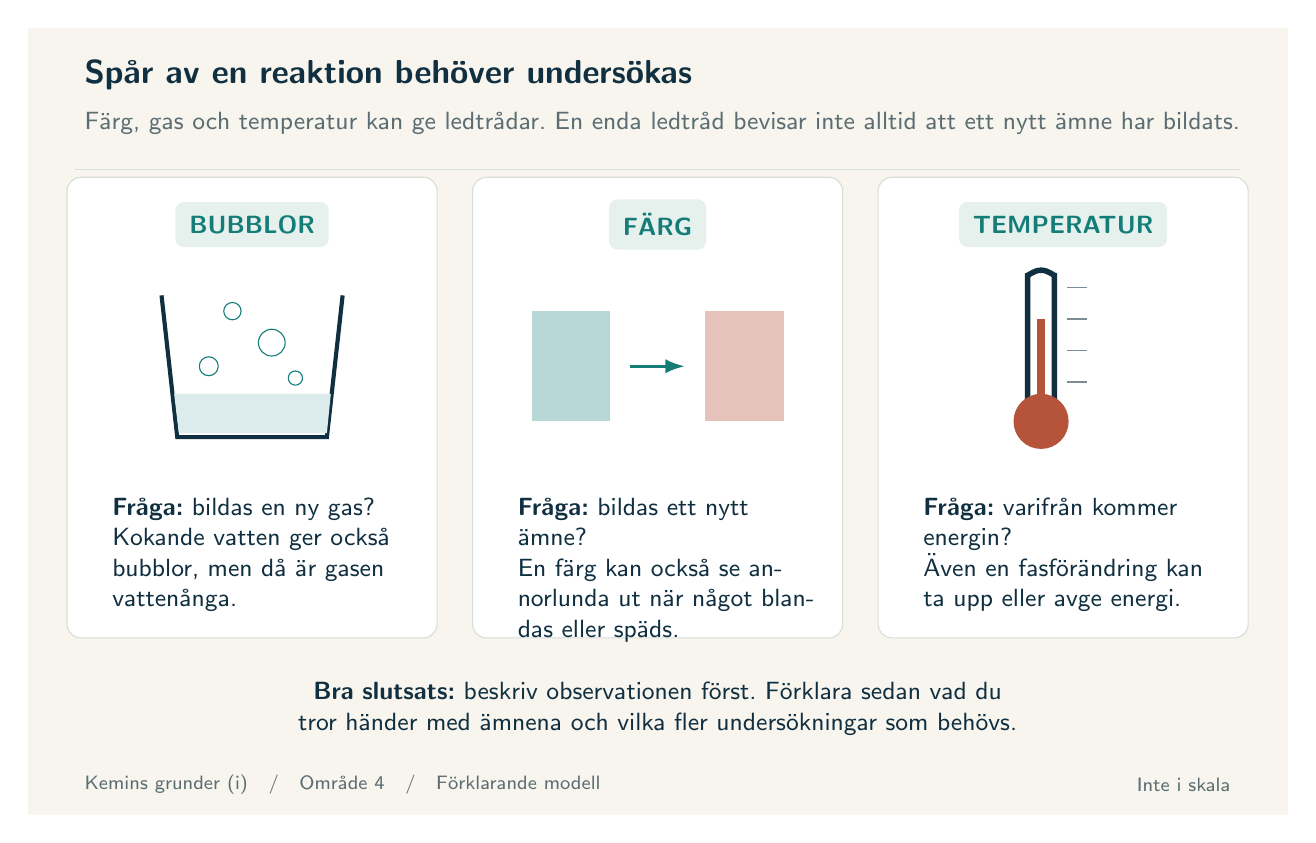
\begin{tikzpicture}[x=1cm,y=1cm]
\path[use as bounding box] (0,0) rectangle (16,10);
\fill[paper] (0,0) rectangle (16,10);
\node[head] at (.6,9.4){Spår av en reaktion behöver undersökas};
\note{.6}{9.05}{14.8}{\textcolor{muted}{Färg, gas och temperatur kan ge ledtrådar. En enda ledtråd bevisar inte alltid att ett nytt ämne har bildats.}}
\draw[line] (.6,8.2)--(15.4,8.2);

\foreach \x in {.5,5.65,10.8}{\panel{\x}{2.25}{4.7}{5.85}}
\node[badge] at (2.85,7.5){BUBBLOR};\node[badge] at (8,7.5){FÄRG};\node[badge] at (13.15,7.5){TEMPERATUR};
\draw[navy,line width=1.5pt] (1.7,6.6)--(1.9,4.8)--(3.8,4.8)--(4,6.6);
\fill[teal!15] (1.86,5.35)--(3.85,5.35)--(3.8,4.85)--(1.92,4.85)--cycle;
\foreach \x/\y/\r in {2.3/5.7/.12,3.1/6/.17,2.6/6.4/.11,3.4/5.55/.09}{\draw[teal] (\x,\y) circle(\r);}
\fill[teal!30] (6.4,5) rectangle(7.4,6.4);\fill[rust!35] (8.6,5) rectangle(9.6,6.4);\draw[arrow] (7.65,5.7)--(8.35,5.7);
\draw[navy,line width=2pt,rounded corners=3pt] (12.7,5.2)--(12.7,6.75) arc(180:0:.17)--(13.04,5.2);\fill[rust] (12.87,5) circle(.35);\draw[rust,line width=3pt] (12.87,5.2)--(12.87,6.3);\foreach \y in {5.5,5.9,6.3,6.7}{\draw[navy!55] (13.2,\y)--(13.45,\y);}
\note{.95}{4.15}{3.8}{\textbf{Fråga:} bildas en ny gas?\par Kokande vatten ger också bubblor, men då är gasen vattenånga.}
\note{6.1}{4.15}{3.8}{\textbf{Fråga:} bildas ett nytt ämne?\par En färg kan också se annorlunda ut när något blandas eller späds.}
\note{11.25}{4.15}{3.8}{\textbf{Fråga:} varifrån kommer energin?\par Även en fasförändring kan ta upp eller avge energi.}
\node[label,text width=14cm] at (8,1.35){\textbf{Bra slutsats:} beskriv observationen först. Förklara sedan vad du tror händer med ämnena och vilka fler undersökningar som behövs.};\node[anchor=west,text=muted,font=\scriptsize] at (.6,.38){Kemins grunder (i)\quad /\quad Område 4\quad /\quad Förklarande modell};
\node[anchor=east,text=muted,font=\scriptsize] at (15.4,.38){Inte i skala};
\end{tikzpicture}\end{document}
